\newpage
\section{Dyson's Equation, Renormalization, RPA and Ladder Approximations}
\subsection{General types of partial sums}
\bgroup
\def\arraystretch{1.}
\begin{table}[H]
\begin{tabular}{cc}
\hline
General type of diagrams summed over                                                                                                                    & Result                                                                                                                            \\ \hline
\begin{tabular}[c]{@{}c@{}}(1) All diagrams containing repeated \\ proper (or 'irreducible') self-energy parts.\\  (Summation is complete)\end{tabular} & Dyson's equation                                                                                                                  \\ \hline
\begin{tabular}[c]{@{}c@{}}(2) All diagrams with "polarization\\  parts" inserted in interaction lines\end{tabular}                                     & \begin{tabular}[c]{@{}c@{}}"dressed", "effective" or\\ "renormalized" interactions\end{tabular}                                   \\\hline
\begin{tabular}[c]{@{}c@{}}(3) All diagrams with self-energy\\ parts' inserted in r ree particle\\ and bole lines\end{tabular}                          & \begin{tabular}[c]{@{}c@{}}"dressed" or "renormalized"\\ particle and bole lines (self-consistent\\ renormalization)\end{tabular} \\\hline
\begin{tabular}[c]{@{}c@{}}(4) All diagrams with 'irreducible\\ vertex parts' inserted in place of\\ a vertex\end{tabular}                              & dressed vertices     \\\hline                                     
\end{tabular}
\end{table}

\subsection{Dyson's Equation}
Let us first define "proper self-energy part" or "irreducible self-energy part". First we define:

\bluep{\textit{Self-energy part}}: Any diagram without incoming and outgoing lines, which can be inserted into a particle or hole line.

\bluep{\textit{Proper or irreducible self-energy part}}: A self-energy part which cannot be broken into two unconnected self-energy parts by removing one particle or hole line. Parts which can be so broken are called 'improper' or 'reducible'.

In general it is possible to sum over all repetitions of all irreducible self-energy parts in a diagram expansion:
\begin{equation}
    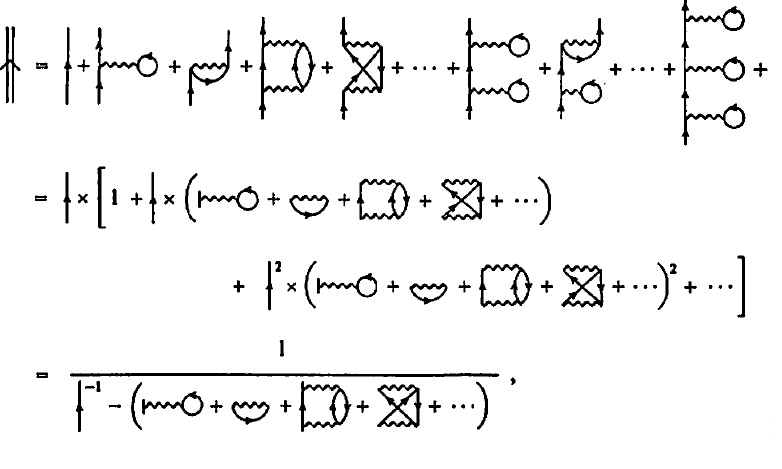
\includegraphics[width=0.8\textwidth]{screenshots/dyson-equation-1.PNG}
    \label{dyson-equation-1}
\end{equation}
or
\begin{equation}
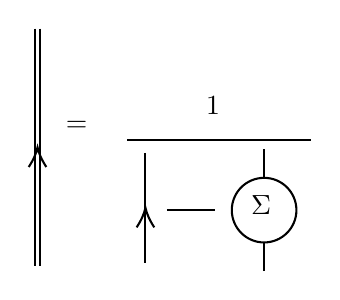
\begin{tikzpicture}[x=0.65pt,y=0.65pt,yscale=-1,xscale=1]
%uncomment if require: \path (0,300); %set diagram left start at 0, and has height of 300

%Straight Lines [id:da5007030956086185] 
\draw    (103.5,63.1) -- (103.5,195)(100.5,63.1) -- (100.5,195) ;
\draw [shift={(102,129.05)}, rotate = 90] [color={rgb, 255:red, 0; green, 0; blue, 0 }  ][line width=0.75]    (10.93,-4.9) .. controls (6.95,-2.3) and (3.31,-0.67) .. (0,0) .. controls (3.31,0.67) and (6.95,2.3) .. (10.93,4.9)   ;
%Straight Lines [id:da27166812193710055] 
\draw    (162,132.1) -- (162,193.1) ;
\draw [shift={(162,162.6)}, rotate = 90] [color={rgb, 255:red, 0; green, 0; blue, 0 }  ][line width=0.75]    (10.93,-4.9) .. controls (6.95,-2.3) and (3.31,-0.67) .. (0,0) .. controls (3.31,0.67) and (6.95,2.3) .. (10.93,4.9)   ;
%Straight Lines [id:da0814970714578146] 
\draw    (151.92,125.1) -- (253.92,125.1) ;
%Shape: Circle [id:dp3367153518929006] 
\draw   (210,163.96) .. controls (210,154.04) and (218.04,146) .. (227.96,146) .. controls (237.88,146) and (245.92,154.04) .. (245.92,163.96) .. controls (245.92,173.88) and (237.88,181.92) .. (227.96,181.92) .. controls (218.04,181.92) and (210,173.88) .. (210,163.96) -- cycle ;
%Straight Lines [id:da44172544983469675] 
\draw    (227.96,146) -- (227.96,130.1) ;
%Straight Lines [id:da9420867165019052] 
\draw    (227.96,197.82) -- (227.96,181.92) ;
%Straight Lines [id:da7785373748433801] 
\draw    (173.96,163.96) -- (200.92,163.96) ;

% Text Node
\draw (219,154) node [anchor=north west][inner sep=0.75pt]    {$\Sigma $};
% Text Node
\draw (194,99) node [anchor=north west][inner sep=0.75pt]    {$1$};
% Text Node
\draw (116,113) node [anchor=north west][inner sep=0.75pt]    {$=$};
\end{tikzpicture}
\label{dyson-eqn-2}
\end{equation}

Translated into functions this becomes:
\begin{equation}G(\mathbf{k}, \omega)=\frac{1}{\omega-\epsilon_{k}-\Sigma(\mathbf{k}, \omega)+i \delta_{k}}\end{equation}
where
\begin{equation}
    -i\Sigma(\mathbf{k},\omega)\equiv\Sigmapart
\end{equation}
It was necessary to restrict the sum to just repeated proper parts. If we had summed over repeated improper parts as well, diagrams would have been counted twice.

Equation (\ref{dyson-equation-1}) or (\ref{dyson-eqn-2}) is called \redp{Dyson's equation} and is the basic equation from which most propagator calculations start. $\Sigma(\mathbf{k},\omega)$ is a \textbf{\redp{generalized "effective field" or "effective potential" which the particle in state $\mathbf{k}$ sees because of its interaction with all the other particles of the system.}} This field is $\omega-$dependent, which describes the motion of the quasi-particle cloud in ($\mathbf{k},t$)-space.

\begin{imp}
The form of (\ref{dyson-eqn-2}) is only valid in the special cases of a system \redp{\textbf{with no external potential and with diagrams calculated in ($\mathbf{k},\omega$)-space.}} A more general form of the Dyson equation which holds whenever the single-particle propagator expansion holds:
\begin{equation}
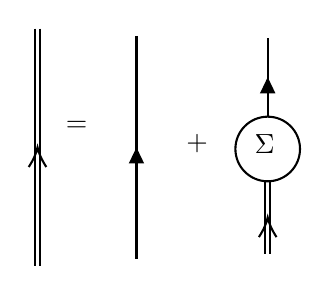
\begin{tikzpicture}[x=0.65pt,y=0.65pt,yscale=-1,xscale=1]
\draw    (103.5,63.1) -- (103.5,195)(100.5,63.1) -- (100.5,195) ;
\draw [shift={(102,129.05)}, rotate = 90] [color={rgb, 255:red, 0; green, 0; blue, 0 }  ][line width=0.75]    (10.93,-4.9) .. controls (6.95,-2.3) and (3.31,-0.67) .. (0,0) .. controls (3.31,0.67) and (6.95,2.3) .. (10.93,4.9)   ;
%Straight Lines [id:da27166812193710055] 
\draw    (157,67.1) -- (157,191.1) ;
\draw [shift={(157,129.1)}, rotate = 90] [fill={rgb, 255:red, 0; green, 0; blue, 0 }  ][line width=0.08]  [draw opacity=0] (8.93,-4.29) -- (0,0) -- (8.93,4.29) -- cycle    ;
%Shape: Circle [id:dp3367153518929006] 
\draw   (212,129.96) .. controls (212,120.04) and (220.04,112) .. (229.96,112) .. controls (239.88,112) and (247.92,120.04) .. (247.92,129.96) .. controls (247.92,139.88) and (239.88,147.92) .. (229.96,147.92) .. controls (220.04,147.92) and (212,139.88) .. (212,129.96) -- cycle ;
%Straight Lines [id:da44172544983469675] 
\draw    (229.96,112) -- (229.96,68.1) ;
\draw [shift={(229.96,90.05)}, rotate = 450] [fill={rgb, 255:red, 0; green, 0; blue, 0 }  ][line width=0.08]  [draw opacity=0] (8.93,-4.29) -- (0,0) -- (8.93,4.29) -- cycle    ;
%Straight Lines [id:da9420867165019052] 
\draw    (228.46,188.1) -- (228.46,147.92)(231.46,188.1) -- (231.46,147.92) ;
\draw [shift={(229.96,168.01)}, rotate = 450] [color={rgb, 255:red, 0; green, 0; blue, 0 }  ][line width=0.75]    (10.93,-4.9) .. controls (6.95,-2.3) and (3.31,-0.67) .. (0,0) .. controls (3.31,0.67) and (6.95,2.3) .. (10.93,4.9)   ;

% Text Node
\draw (221,120) node [anchor=north west][inner sep=0.75pt]    {$\Sigma $};
% Text Node
\draw (116,113) node [anchor=north west][inner sep=0.75pt]    {$=$};
% Text Node
\draw (183,120) node [anchor=north west][inner sep=0.75pt]    {$+$};


\end{tikzpicture}
\label{generalized-dyson-eqn}
\end{equation}
\end{imp}
Equation (\ref{generalized-dyson-eqn}) boils down to (\ref{dyson-eqn-2}) for a system without external potential because the value of each diagram is the product of the values of its parts:
\begin{equation}
   \tikzset{every picture/.style={line width=0.75pt}} %set default line width to 0.75pt        
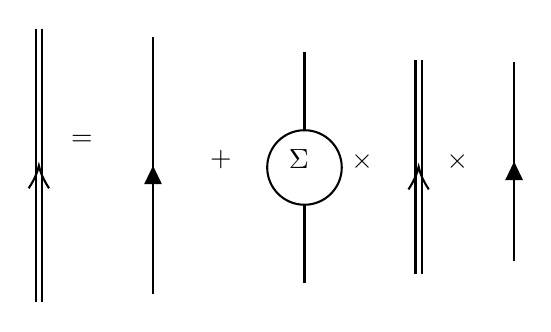
\begin{tikzpicture}[x=0.75pt,y=0.75pt,yscale=-1,xscale=1]
%uncomment if require: \path (0,300); %set diagram left start at 0, and has height of 300
\draw    (103.5,63.1) -- (103.5,195)(100.5,63.1) -- (100.5,195) ;
\draw [shift={(102,129.05)}, rotate = 90] [color={rgb, 255:red, 0; green, 0; blue, 0 }  ][line width=0.75]    (10.93,-4.9) .. controls (6.95,-2.3) and (3.31,-0.67) .. (0,0) .. controls (3.31,0.67) and (6.95,2.3) .. (10.93,4.9)   ;
%Straight Lines [id:da27166812193710055] 
\draw    (157,67.1) -- (157,191.1) ;
\draw [shift={(157,129.1)}, rotate = 90] [fill={rgb, 255:red, 0; green, 0; blue, 0 }  ][line width=0.08]  [draw opacity=0] (8.93,-4.29) -- (0,0) -- (8.93,4.29) -- cycle    ;
%Shape: Circle [id:dp3367153518929006] 
\draw   (212,129.96) .. controls (212,120.04) and (220.04,112) .. (229.96,112) .. controls (239.88,112) and (247.92,120.04) .. (247.92,129.96) .. controls (247.92,139.88) and (239.88,147.92) .. (229.96,147.92) .. controls (220.04,147.92) and (212,139.88) .. (212,129.96) -- cycle ;
%Straight Lines [id:da44172544983469675] 
\draw    (330.96,175.1) -- (330.96,79.1) ;
\draw [shift={(330.96,127.1)}, rotate = 450] [fill={rgb, 255:red, 0; green, 0; blue, 0 }  ][line width=0.08]  [draw opacity=0] (8.93,-4.29) -- (0,0) -- (8.93,4.29) -- cycle    ;
%Straight Lines [id:da9420867165019052] 
\draw    (283.46,181.1) -- (283.46,78.1)(286.46,181.1) -- (286.46,78.1) ;
\draw [shift={(284.96,129.6)}, rotate = 450] [color={rgb, 255:red, 0; green, 0; blue, 0 }  ][line width=0.75]    (10.93,-4.9) .. controls (6.95,-2.3) and (3.31,-0.67) .. (0,0) .. controls (3.31,0.67) and (6.95,2.3) .. (10.93,4.9)   ;
%Straight Lines [id:da9087104573290277] 
\draw    (229.96,74.1) -- (229.96,112) ;
%Straight Lines [id:da256765400607896] 
\draw    (229.96,147.92) -- (229.96,185.82) ;
\draw (221,120) node [anchor=north west][inner sep=0.75pt]    {$\Sigma $};
% Text Node
\draw (116,113) node [anchor=north west][inner sep=0.75pt]    {$=$};
% Text Node
\draw (183,120) node [anchor=north west][inner sep=0.75pt]    {$+$};
% Text Node
\draw (251,121) node [anchor=north west][inner sep=0.75pt]    {$\times $};
% Text Node
\draw (297,121) node [anchor=north west][inner sep=0.75pt]    {$\times $};


\end{tikzpicture} 
\end{equation}
or
\begin{equation}G(\mathbf{k}, \omega)=G_{0}(\mathbf{k}, \omega)+G(\mathbf{k}, \omega) \Sigma(\mathbf{k}, \omega) G_{0}(\mathbf{k}, \omega)\end{equation}
\redp{Equation (\ref{generalized-dyson-eqn}) is also valid when the diagrams do not factor}. For example, in $(\mathbf{k},t)$-space we find
\begin{equation}\begin{aligned}
i G\left(\mathbf{k}, t_{2}-t_{1}\right)=i &G_{0}\left(\mathbf{k}, t_{2}-t_{1}\right)+\\
&+\iint d t^{\prime} d t^{\prime \prime} i G_{0}\left(\mathbf{k}, t_{2}-t^{\prime \prime}\right)(-i) \Sigma\left(\mathbf{k}, t^{\prime \prime}-t^{\prime}\right) i G\left(\mathbf{k}, t^{\prime}-t_{1}\right)
\end{aligned}\end{equation}

Another example of (\ref{generalized-dyson-eqn}) is the case of a system with an external potential. Then
\begin{equation}\begin{aligned}
i G\left(k_{2}, k_{1} ; \omega\right)=i G_{0}&\left(k_{2}, \omega\right) \delta_{k_{2} k_{1}}+& \\
&+\sum_{k, k^{\prime}} i G_{0}\left(k_{2}, \omega\right) \delta_{k_{2} k^{\prime}}(-i) \Sigma\left(k^{\prime}, k ; \omega\right) i G\left(k, k_{1} ; \omega\right)
\end{aligned}\end{equation}
Note that now anomalous graphs must be included

\subsection{Quasi particles in low-density Fermi system (ladder approximation)}
We now describe the theory of Galitski for a system of particles interacting by means of short-range repulsive forces having range $a$, and with average distance between particles $r_0$. By 'low density' is meant that $a / r_{0} \ll 1 .$ This can also be stated in terms of $k_{F}$ since $n,$ the number of particles/cm $^{3}$ is equal to $\frac{1}{3} \pi^{-2} k_{F}^{3}$(\ref{N0-kF-relation}) and $n=1 / r_{0}^{3}$ so $1 / r_{0} \sim k_{F} .$ Hence the low-density criterion is that $k_{F} a \ll 1 .$ Such a theory can be applied in a qualitative way to the case of nuclear matter, where $a / r_{0} \sim \frac{1}{3},$ provided we neglect the attractive part of the nuclear potential.

Let us first analyse which self-energy diagrams are the most important ones. We first notice that whenever there is a hole line, labelled by $\mathbf{p}$, there is an associated $\int d^3\mathbf{p}$ over $|\mathbf{p}|<k_F$. Particle lines have $\int d^3\mathbf{p}$ over $|\mathbf{p}|>k_F$. As mentioned before, $n\approx k^3_F$, so low density corresponds to low $k_F$. In low-density case, the contribution from the hole line integrals is negligible compared to those from particle line integral. Therefore, the dominant diagrams will be those with the least number of hole lines. We find for the sum of graphs containing just one hole line the following:
\begin{equation}
    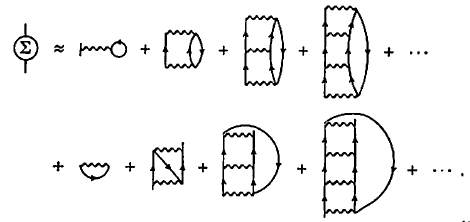
\includegraphics[width=0.8\textwidth]{screenshots/ladder-approx.PNG}
    \label{ladder-approx}
\end{equation}
These are called "\bluep{ladder graphs}". The sum of ladder graphs may be carried out with the aid of "$K$"-matrix. This is defined by:
\begin{equation}
    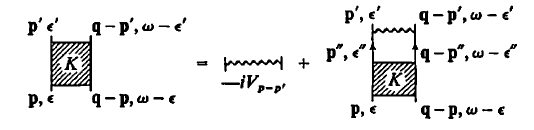
\includegraphics[width=0.8\textwidth]{screenshots/K-matrix.PNG}
    \label{K-matrix-defi}
\end{equation}
which gives
\begin{equation}
\begin{aligned}
K\left(\mathbf{p}^{\prime} \boldsymbol{\epsilon}^{\prime}, \mathbf{p}, \epsilon ; \mathbf{q}, \omega\right)=V_{p-p^{\prime}}+i \int \frac{d^{3} \mathbf{p}^{\prime\prime} d \epsilon^{\prime \prime}}{(2 \pi)^{4}} V_{p^{\prime\prime}-p^{\prime}} &G_{0}^{+}\left(\mathbf{p}^{\prime \prime}, \epsilon^{\prime \prime}\right) G_{0}^{+}\left(\mathbf{q}-\mathbf{p}^{\prime \prime}, \omega-\epsilon^{\prime \prime}\right)\times\\
&K(\mathbf{p}^{\prime\prime},\epsilon^{\prime\prime},\mathbf{p},\epsilon;\mathbf{q},\omega)
\end{aligned}
\end{equation}

\subsection{Quasi particles In high-density electron gas (random phase approximation)}
The electron gas was introduced as a theoretical metal consisting of N electrons moving against a smeared-out positive charge background. At zero temperature, the gas is characterized by a single parameter, \textbf{the average distance between electrons, $r_s$}. More precisely, $r_s$ is given by
\begin{equation}\frac{1}{n}\left(\frac{\mathrm{cm}^{3}}{\mathrm{electron}}\right)=\frac{4}{3} \pi\left(r_{s} a_{0}\right)^{3}\end{equation}
where $n=$ electron density, and $a_{0}=$ Bohr radius $=\hbar^{2} / m e^{2}$.

It is important to observe that the low density system with long-range interaction, like the electron gas, is physically different from the low-density system with short-range interaction, like nuclear matter. Hence ladder approximation is not applicable here.

The Hamiltonian for the electron gas in the smeared out positive background is given by
\begin{equation}
\begin{aligned}
H=\sum_{k} &\epsilon_{k} c_{k}^{\dagger} c_{k}+\frac{1}{2} \sum_{k l m n} V_{k l m n} c^{\dagger}_l c_{k} c_{m} c_{n}\\
& H_{\substack{positive\\background}}+H_{\substack{electron-positive\\background}}
\end{aligned}
\end{equation}
This equation may be simplified since the $V_0$ part of the second sum can be used to cancel the last two terms as follows: The $V_0$ may be evaluated as (dropping spin factors for simplicity):
\begin{equation}V_{0}=V_{k l k l}=\frac{1}{\Omega^{2}} \int d^{3} \mathbf{r} d^{3} \mathbf{r}^{\prime} \frac{e^{2}}{\left|\mathbf{r}-\mathbf{r}^{\prime}\right|}\end{equation}
According to the commutation rule of $[c^{\dagger}_l,c_k]_+=\delta_{lk}$, we have $V_0$ as:
\begin{equation}\begin{aligned}
\frac{V_{0}}{2} \sum_{k l} c_{l}^{\dagger} c_{k}^{\dagger} c_{k} c_{l} &=\frac{V_{0}}{2} \sum_{k=1}^{+} c_{l}^{\dagger} c_{l} c_{k}^{\dagger} c_{k}-\frac{V_{0}}{2} \sum_{k} c_{k}^{\dagger} c_{k} \\
&=\frac{V_{0}}{2}\left(N^{2}-N\right)=\frac{1}{2} \frac{N^{2} e^{2}}{\Omega^{2}} \int \frac{d^{3} r d^{3} \mathbf{r}^{\prime}}{\left|\mathbf{r}-\mathbf{r}^{\prime}\right|}
\end{aligned}
\label{static-self-energy}
\end{equation}
where we used the fact of $N^2\gg N$.(\ref{static-self-energy}) is just the self-energy of a static uniform negative charge distribution. \bluep{The static positive background is exactly equal to (\ref{static-self-energy}) while the electron-background term gives a contribution which is twice (\ref{static-self-energy}) and of opposite sign.}(i.e., $V_{electron-positive}=\frac{N^{2} eZ}{\Omega^{2}} \int \frac{d^{3} \mathbf{r} d^{3} \mathbf{r}^{\prime}}{\left|\mathbf{r}-\mathbf{r}^{\prime}\right|}$. We don't have $1/2$ here because electrons and are distinguiable from positive background). That is,
\begin{equation}H=\sum_{k} \epsilon_{k} c_{k}^{\dagger} c_{k}+\frac{1}{2} \sum_{\substack{g, m, n \\ (q \neq 0)}} V_{q} c_{n-q}^{\dagger} c_{m+q}^{\dagger} c_{m} c_{n}\end{equation}
We can now find quasi particles in the electron gas, using (\ref{dyson-eqn-2}) and (\ref{V-klmn-with-spin}). A typical irreducible self-energy part is:

\begin{equation}
    \begin{aligned}
    &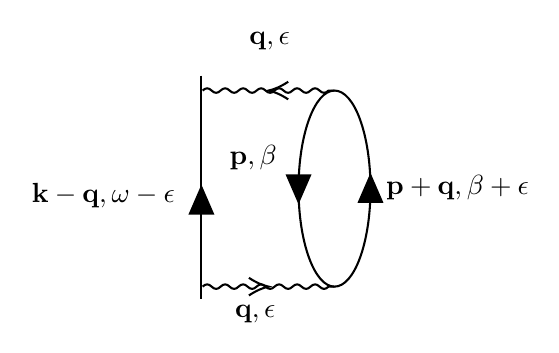
\begin{tikzpicture}[x=0.65pt,y=0.65pt,yscale=-1,xscale=1]
%uncomment if require: \path (0,300); %set diagram left start at 0, and has height of 300

%Straight Lines [id:da27166812193710055] 
\draw    (157,67.1) -- (157,191.1) ;
%Shape: Ellipse [id:dp447508023627581] 
\draw   (231,75.38) .. controls (242.05,75.38) and (251,99.78) .. (251,129.88) .. controls (251,159.98) and (242.05,184.38) .. (231,184.38) .. controls (219.95,184.38) and (211,159.98) .. (211,129.88) .. controls (211,99.78) and (219.95,75.38) .. (231,75.38) -- cycle ;
%Shape: Triangle [id:dp8599343851274321] 
\draw  [fill={rgb, 255:red, 0; green, 0; blue, 0 }  ,fill opacity=1 ] (251,122.57) -- (257.34,137.19) -- (244.66,137.19) -- cycle ;
%Shape: Triangle [id:dp08374775280444868] 
\draw  [fill={rgb, 255:red, 0; green, 0; blue, 0 }  ,fill opacity=1 ] (157,129.1) -- (163.34,143.72) -- (150.66,143.72) -- cycle ;
%Shape: Triangle [id:dp4084243696074741] 
\draw  [fill={rgb, 255:red, 0; green, 0; blue, 0 }  ,fill opacity=1 ] (211,137.19) -- (204.66,122.57) -- (217.34,122.57) -- cycle ;
%Straight Lines [id:da09326610557496029] 
\draw    (157.68,184.38) .. controls (159.35,182.71) and (161.01,182.71) .. (162.68,184.38) .. controls (164.35,186.05) and (166.01,186.05) .. (167.68,184.38) .. controls (169.35,182.71) and (171.01,182.71) .. (172.68,184.38) .. controls (174.35,186.05) and (176.01,186.05) .. (177.68,184.38) .. controls (179.35,182.71) and (181.01,182.71) .. (182.68,184.38) .. controls (184.35,186.05) and (186.01,186.05) .. (187.68,184.38) .. controls (189.35,182.71) and (191.01,182.71) .. (192.68,184.38) .. controls (194.35,186.05) and (196.01,186.05) .. (197.68,184.38) .. controls (199.35,182.71) and (201.01,182.71) .. (202.68,184.38) .. controls (204.35,186.05) and (206.01,186.05) .. (207.68,184.38) .. controls (209.35,182.71) and (211.01,182.71) .. (212.68,184.38) .. controls (214.35,186.05) and (216.01,186.05) .. (217.68,184.38) .. controls (219.35,182.71) and (221.01,182.71) .. (222.68,184.38) .. controls (224.35,186.05) and (226.01,186.05) .. (227.68,184.38) -- (231,184.38) -- (231,184.38) ;
\draw [shift={(194.34,184.38)}, rotate = 180] [color={rgb, 255:red, 0; green, 0; blue, 0 }  ][line width=0.75]    (10.93,-4.9) .. controls (6.95,-2.3) and (3.31,-0.67) .. (0,0) .. controls (3.31,0.67) and (6.95,2.3) .. (10.93,4.9)   ;
%Straight Lines [id:da8741947169845137] 
\draw    (157.68,75.38) .. controls (159.35,73.71) and (161.01,73.71) .. (162.68,75.38) .. controls (164.35,77.05) and (166.01,77.05) .. (167.68,75.38) .. controls (169.35,73.71) and (171.01,73.71) .. (172.68,75.38) .. controls (174.35,77.05) and (176.01,77.05) .. (177.68,75.38) .. controls (179.35,73.71) and (181.01,73.71) .. (182.68,75.38) .. controls (184.35,77.05) and (186.01,77.05) .. (187.68,75.38) .. controls (189.35,73.71) and (191.01,73.71) .. (192.68,75.38) .. controls (194.35,77.05) and (196.01,77.05) .. (197.68,75.38) .. controls (199.35,73.71) and (201.01,73.71) .. (202.68,75.38) .. controls (204.35,77.05) and (206.01,77.05) .. (207.68,75.38) .. controls (209.35,73.71) and (211.01,73.71) .. (212.68,75.38) .. controls (214.35,77.05) and (216.01,77.05) .. (217.68,75.38) .. controls (219.35,73.71) and (221.01,73.71) .. (222.68,75.38) .. controls (224.35,77.05) and (226.01,77.05) .. (227.68,75.38) -- (231,75.38) -- (231,75.38) ;
\draw [shift={(194.34,75.38)}, rotate = 0] [color={rgb, 255:red, 0; green, 0; blue, 0 }  ][line width=0.75]    (10.93,-4.9) .. controls (6.95,-2.3) and (3.31,-0.67) .. (0,0) .. controls (3.31,0.67) and (6.95,2.3) .. (10.93,4.9)   ;

% Text Node
\draw (182,41) node [anchor=north west][inner sep=0.75pt]    {$\mathbf{q} ,\epsilon $};
% Text Node
\draw (174,193) node [anchor=north west][inner sep=0.75pt]    {$\mathbf{q} ,\epsilon $};
% Text Node
\draw (61,125) node [anchor=north west][inner sep=0.75pt]    {$\mathbf{k} -\mathbf{q} ,\omega -\epsilon $};
% Text Node
\draw (258,121) node [anchor=north west][inner sep=0.75pt]    {$\mathbf{p} +\mathbf{q} ,\beta +\epsilon $};
% Text Node
\draw (171,104) node [anchor=north west][inner sep=0.75pt]    {$\mathbf{p} ,\beta $};


\end{tikzpicture}\\
&=(-1) \sum_{\mathbf{q,p}} \int \frac{d \epsilon d \beta}{(2 \pi)^{2}} i G_{0}(k-q, \omega-\epsilon) \times i G_{0}(q+p, \beta+\epsilon) \times\\
&i G_{0}(\mathbf{p}, \beta) \times \frac{\left(4 \pi e^{2}\right)^{2}}{\Omega^{2} q^{4}}
    \end{aligned}
\end{equation}
Changing from a sum over $q$ to an integral reveals that the above expression diverges at $\mathbf{q}=0$ because of the $q^{4}$ in the denominator so that
\begin{equation}
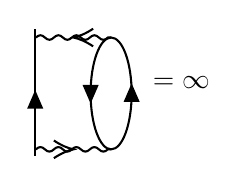
\begin{tikzpicture}[x=0.65pt,y=0.65pt,yscale=-1,xscale=1]
%uncomment if require: \path (0,300); %set diagram left start at 0, and has height of 300

%Straight Lines [id:da27166812193710055] 
\draw    (154.27,120.38) -- (154.27,191.1) ;
%Shape: Ellipse [id:dp447508023627581] 
\draw   (196.48,125.11) .. controls (202.78,125.11) and (207.88,139.02) .. (207.88,156.19) .. controls (207.88,173.35) and (202.78,187.27) .. (196.48,187.27) .. controls (190.18,187.27) and (185.07,173.35) .. (185.07,156.19) .. controls (185.07,139.02) and (190.18,125.11) .. (196.48,125.11) -- cycle ;
%Shape: Triangle [id:dp8599343851274321] 
\draw  [fill={rgb, 255:red, 0; green, 0; blue, 0 }  ,fill opacity=1 ] (207.88,152.02) -- (211.5,160.36) -- (204.27,160.36) -- cycle ;
%Shape: Triangle [id:dp08374775280444868] 
\draw  [fill={rgb, 255:red, 0; green, 0; blue, 0 }  ,fill opacity=1 ] (154.27,155.74) -- (157.89,164.08) -- (150.66,164.08) -- cycle ;
%Shape: Triangle [id:dp4084243696074741] 
\draw  [fill={rgb, 255:red, 0; green, 0; blue, 0 }  ,fill opacity=1 ] (185.07,160.36) -- (181.45,152.02) -- (188.69,152.02) -- cycle ;
%Straight Lines [id:da09326610557496029] 
\draw    (154.66,187.27) .. controls (156.33,185.6) and (157.99,185.6) .. (159.66,187.27) .. controls (161.33,188.94) and (162.99,188.94) .. (164.66,187.27) .. controls (166.33,185.6) and (167.99,185.6) .. (169.66,187.27) .. controls (171.33,188.94) and (172.99,188.94) .. (174.66,187.27) .. controls (176.33,185.6) and (177.99,185.6) .. (179.66,187.27) .. controls (181.33,188.94) and (182.99,188.94) .. (184.66,187.27) .. controls (186.33,185.6) and (187.99,185.6) .. (189.66,187.27) .. controls (191.33,188.94) and (192.99,188.94) .. (194.66,187.27) -- (196.48,187.27) -- (196.48,187.27) ;
\draw [shift={(175.57,187.27)}, rotate = 180] [color={rgb, 255:red, 0; green, 0; blue, 0 }  ][line width=0.75]    (10.93,-4.9) .. controls (6.95,-2.3) and (3.31,-0.67) .. (0,0) .. controls (3.31,0.67) and (6.95,2.3) .. (10.93,4.9)   ;
%Straight Lines [id:da8741947169845137] 
\draw    (154.66,125.11) .. controls (156.33,123.44) and (157.99,123.44) .. (159.66,125.11) .. controls (161.33,126.78) and (162.99,126.78) .. (164.66,125.11) .. controls (166.33,123.44) and (167.99,123.44) .. (169.66,125.11) .. controls (171.33,126.78) and (172.99,126.78) .. (174.66,125.11) .. controls (176.33,123.44) and (177.99,123.44) .. (179.66,125.11) .. controls (181.33,126.78) and (182.99,126.78) .. (184.66,125.11) .. controls (186.33,123.44) and (187.99,123.44) .. (189.66,125.11) .. controls (191.33,126.78) and (192.99,126.78) .. (194.66,125.11) -- (196.48,125.11) -- (196.48,125.11) ;
\draw [shift={(175.57,125.11)}, rotate = 0] [color={rgb, 255:red, 0; green, 0; blue, 0 }  ][line width=0.75]    (10.93,-4.9) .. controls (6.95,-2.3) and (3.31,-0.67) .. (0,0) .. controls (3.31,0.67) and (6.95,2.3) .. (10.93,4.9)   ;

% Text Node
\draw (218,145) node [anchor=north west][inner sep=0.75pt]    {$=\infty $};


\end{tikzpicture}
\end{equation}

However, the situation is saved by the partial summation method as follows: First we observe that \bluep{each term in the self-energy is proportional to some power of $r_s$}. To see this, we reproduce the integral for a 2-nd order self-energy part as:
\begin{equation}
    \begin{aligned}
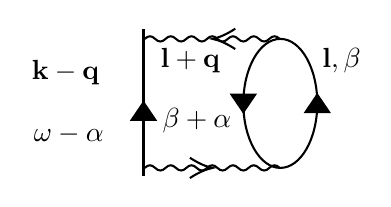
\begin{tikzpicture}[x=0.75pt,y=0.75pt,yscale=-1,xscale=1]
%uncomment if require: \path (0,300); %set diagram left start at 0, and has height of 300

%Straight Lines [id:da27166812193710055] 
\draw    (156.31,120.38) -- (156.31,191.1) ;
%Shape: Ellipse [id:dp447508023627581] 
\draw   (222.22,125.11) .. controls (232.06,125.11) and (240.03,139.02) .. (240.03,156.19) .. controls (240.03,173.35) and (232.06,187.27) .. (222.22,187.27) .. controls (212.38,187.27) and (204.41,173.35) .. (204.41,156.19) .. controls (204.41,139.02) and (212.38,125.11) .. (222.22,125.11) -- cycle ;
%Shape: Triangle [id:dp8599343851274321] 
\draw  [fill={rgb, 255:red, 0; green, 0; blue, 0 }  ,fill opacity=1 ] (240.03,152.02) -- (245.68,160.36) -- (234.39,160.36) -- cycle ;
%Shape: Triangle [id:dp08374775280444868] 
\draw  [fill={rgb, 255:red, 0; green, 0; blue, 0 }  ,fill opacity=1 ] (156.31,155.74) -- (161.96,164.08) -- (150.66,164.08) -- cycle ;
%Shape: Triangle [id:dp4084243696074741] 
\draw  [fill={rgb, 255:red, 0; green, 0; blue, 0 }  ,fill opacity=1 ] (204.41,160.36) -- (198.76,152.02) -- (210.05,152.02) -- cycle ;
%Straight Lines [id:da09326610557496029] 
\draw    (156.92,187.27) .. controls (158.59,185.6) and (160.25,185.6) .. (161.92,187.27) .. controls (163.59,188.94) and (165.25,188.94) .. (166.92,187.27) .. controls (168.59,185.6) and (170.25,185.6) .. (171.92,187.27) .. controls (173.59,188.94) and (175.25,188.94) .. (176.92,187.27) .. controls (178.59,185.6) and (180.25,185.6) .. (181.92,187.27) .. controls (183.59,188.94) and (185.25,188.94) .. (186.92,187.27) .. controls (188.59,185.6) and (190.25,185.6) .. (191.92,187.27) .. controls (193.59,188.94) and (195.25,188.94) .. (196.92,187.27) .. controls (198.59,185.6) and (200.25,185.6) .. (201.92,187.27) .. controls (203.59,188.94) and (205.25,188.94) .. (206.92,187.27) .. controls (208.59,185.6) and (210.25,185.6) .. (211.92,187.27) .. controls (213.59,188.94) and (215.25,188.94) .. (216.92,187.27) .. controls (218.59,185.6) and (220.25,185.6) .. (221.92,187.27) -- (222.22,187.27) -- (222.22,187.27) ;
\draw [shift={(189.57,187.27)}, rotate = 180] [color={rgb, 255:red, 0; green, 0; blue, 0 }  ][line width=0.75]    (10.93,-4.9) .. controls (6.95,-2.3) and (3.31,-0.67) .. (0,0) .. controls (3.31,0.67) and (6.95,2.3) .. (10.93,4.9)   ;
%Straight Lines [id:da8741947169845137] 
\draw    (156.92,125.11) .. controls (158.59,123.44) and (160.25,123.44) .. (161.92,125.11) .. controls (163.59,126.78) and (165.25,126.78) .. (166.92,125.11) .. controls (168.59,123.44) and (170.25,123.44) .. (171.92,125.11) .. controls (173.59,126.78) and (175.25,126.78) .. (176.92,125.11) .. controls (178.59,123.44) and (180.25,123.44) .. (181.92,125.11) .. controls (183.59,126.78) and (185.25,126.78) .. (186.92,125.11) .. controls (188.59,123.44) and (190.25,123.44) .. (191.92,125.11) .. controls (193.59,126.78) and (195.25,126.78) .. (196.92,125.11) .. controls (198.59,123.44) and (200.25,123.44) .. (201.92,125.11) .. controls (203.59,126.78) and (205.25,126.78) .. (206.92,125.11) .. controls (208.59,123.44) and (210.25,123.44) .. (211.92,125.11) .. controls (213.59,126.78) and (215.25,126.78) .. (216.92,125.11) .. controls (218.59,123.44) and (220.25,123.44) .. (221.92,125.11) -- (222.22,125.11) -- (222.22,125.11) ;
\draw [shift={(189.57,125.11)}, rotate = 0] [color={rgb, 255:red, 0; green, 0; blue, 0 }  ][line width=0.75]    (10.93,-4.9) .. controls (6.95,-2.3) and (3.31,-0.67) .. (0,0) .. controls (3.31,0.67) and (6.95,2.3) .. (10.93,4.9)   ;

% Text Node
\draw (101,134) node [anchor=north west][inner sep=0.75pt]    {$\mathbf{k-q}$};
% Text Node
\draw (241,128) node [anchor=north west][inner sep=0.75pt]    {$\mathbf{l} ,\beta $};
% Text Node
\draw (163,128) node [anchor=north west][inner sep=0.75pt]    {$\mathbf{l} +\mathbf{q}$};
% Text Node
\draw (163.96,157.08) node [anchor=north west][inner sep=0.75pt]    {$\beta +\alpha $};
% Text Node
\draw (101.96,165.08) node [anchor=north west][inner sep=0.75pt]    {$\omega -\alpha $};


\end{tikzpicture}=&\int \frac{d^{3} \mathbf{q}}{(2 \pi)^{3}} \int \frac{d \alpha}{2 \pi}\left(-i V_{q}\right)^{2} \frac{i}{\omega-\alpha-\epsilon_{k-q}+i \delta_{k-q}}\times\\
&\times\left[-i \pi_{0}^{A}(\mathbf{q}, \alpha)+i \pi_{0}^{B}(\mathbf{q}, \alpha)\right]
    \end{aligned}
\end{equation}
Let us first examine the $\pi^A_0$-term:
\begin{equation}
    \begin{aligned}
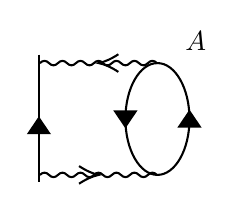
\begin{tikzpicture}[x=0.65pt,y=0.65pt,yscale=-1,xscale=1]
\draw    (351.31,56.38) -- (351.31,127.1) ;
%Shape: Ellipse [id:dp8949329493509471] 
\draw   (417.22,61.11) .. controls (427.06,61.11) and (435.03,75.02) .. (435.03,92.19) .. controls (435.03,109.35) and (427.06,123.27) .. (417.22,123.27) .. controls (407.38,123.27) and (399.41,109.35) .. (399.41,92.19) .. controls (399.41,75.02) and (407.38,61.11) .. (417.22,61.11) -- cycle ;
%Shape: Triangle [id:dp28554712188672693] 
\draw  [fill={rgb, 255:red, 0; green, 0; blue, 0 }  ,fill opacity=1 ] (435.03,88.02) -- (440.68,96.36) -- (429.39,96.36) -- cycle ;
%Shape: Triangle [id:dp06541673528621583] 
\draw  [fill={rgb, 255:red, 0; green, 0; blue, 0 }  ,fill opacity=1 ] (351.31,91.74) -- (356.96,100.08) -- (345.66,100.08) -- cycle ;
%Shape: Triangle [id:dp14671184245926794] 
\draw  [fill={rgb, 255:red, 0; green, 0; blue, 0 }  ,fill opacity=1 ] (399.41,96.36) -- (393.76,88.02) -- (405.05,88.02) -- cycle ;
%Straight Lines [id:da9262621165150392] 
\draw    (351.92,123.27) .. controls (353.59,121.6) and (355.25,121.6) .. (356.92,123.27) .. controls (358.59,124.94) and (360.25,124.94) .. (361.92,123.27) .. controls (363.59,121.6) and (365.25,121.6) .. (366.92,123.27) .. controls (368.59,124.94) and (370.25,124.94) .. (371.92,123.27) .. controls (373.59,121.6) and (375.25,121.6) .. (376.92,123.27) .. controls (378.59,124.94) and (380.25,124.94) .. (381.92,123.27) .. controls (383.59,121.6) and (385.25,121.6) .. (386.92,123.27) .. controls (388.59,124.94) and (390.25,124.94) .. (391.92,123.27) .. controls (393.59,121.6) and (395.25,121.6) .. (396.92,123.27) .. controls (398.59,124.94) and (400.25,124.94) .. (401.92,123.27) .. controls (403.59,121.6) and (405.25,121.6) .. (406.92,123.27) .. controls (408.59,124.94) and (410.25,124.94) .. (411.92,123.27) .. controls (413.59,121.6) and (415.25,121.6) .. (416.92,123.27) -- (417.22,123.27) -- (417.22,123.27) ;
\draw [shift={(384.57,123.27)}, rotate = 180] [color={rgb, 255:red, 0; green, 0; blue, 0 }  ][line width=0.75]    (10.93,-4.9) .. controls (6.95,-2.3) and (3.31,-0.67) .. (0,0) .. controls (3.31,0.67) and (6.95,2.3) .. (10.93,4.9)   ;
%Straight Lines [id:da8988287550837569] 
\draw    (351.92,61.11) .. controls (353.59,59.44) and (355.25,59.44) .. (356.92,61.11) .. controls (358.59,62.78) and (360.25,62.78) .. (361.92,61.11) .. controls (363.59,59.44) and (365.25,59.44) .. (366.92,61.11) .. controls (368.59,62.78) and (370.25,62.78) .. (371.92,61.11) .. controls (373.59,59.44) and (375.25,59.44) .. (376.92,61.11) .. controls (378.59,62.78) and (380.25,62.78) .. (381.92,61.11) .. controls (383.59,59.44) and (385.25,59.44) .. (386.92,61.11) .. controls (388.59,62.78) and (390.25,62.78) .. (391.92,61.11) .. controls (393.59,59.44) and (395.25,59.44) .. (396.92,61.11) .. controls (398.59,62.78) and (400.25,62.78) .. (401.92,61.11) .. controls (403.59,59.44) and (405.25,59.44) .. (406.92,61.11) .. controls (408.59,62.78) and (410.25,62.78) .. (411.92,61.11) .. controls (413.59,59.44) and (415.25,59.44) .. (416.92,61.11) -- (417.22,61.11) -- (417.22,61.11) ;
\draw [shift={(384.57,61.11)}, rotate = 0] [color={rgb, 255:red, 0; green, 0; blue, 0 }  ][line width=0.75]    (10.93,-4.9) .. controls (6.95,-2.3) and (3.31,-0.67) .. (0,0) .. controls (3.31,0.67) and (6.95,2.3) .. (10.93,4.9)   ;

% Text Node
\draw (431,42) node [anchor=north west][inner sep=0.75pt]    {$A$};


\end{tikzpicture}=&(-2) \int \frac{d^{3} q}{(2 \pi)^{3}} V_{q^{2}} \underset{\substack{l<k_F\\|l+q|>k_F}}{\int \frac{d^{3} \mathbf{l}}{(2 \pi)^{3}}} \int \frac{d \alpha}{2 \pi} \\
&\times \frac{1}{\omega-\alpha-\epsilon_{k-q}+i \delta_{k-q}} \times \frac{1}{\epsilon_{t}-\epsilon_{l+q}+\alpha+i \delta}
    \end{aligned}
\end{equation}
The poles here, in the $\alpha-$integration are at
$$\begin{array}{l}
\alpha=-\epsilon_{l}+\epsilon_{l+q}-i \delta \\
\alpha=\omega-\epsilon_{k-q}+i \delta_{k-q}
\end{array}$$
The integration is done by contours just as before. We see that $|\mathbf{k}-\mathbf{q}|$ must be $>k_{F},$ otherwise both poles are in the lower half-plane and we get zero.(\redp{remember the contour integration is always finished in a \textbf{counter-clockwise} fashion}) The result is
\begin{equation}
    \begin{aligned}
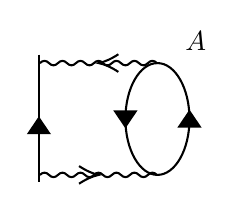
\begin{tikzpicture}[x=0.65pt,y=0.65pt,yscale=-1,xscale=1]
\draw    (351.31,56.38) -- (351.31,127.1) ;
%Shape: Ellipse [id:dp8949329493509471] 
\draw   (417.22,61.11) .. controls (427.06,61.11) and (435.03,75.02) .. (435.03,92.19) .. controls (435.03,109.35) and (427.06,123.27) .. (417.22,123.27) .. controls (407.38,123.27) and (399.41,109.35) .. (399.41,92.19) .. controls (399.41,75.02) and (407.38,61.11) .. (417.22,61.11) -- cycle ;
%Shape: Triangle [id:dp28554712188672693] 
\draw  [fill={rgb, 255:red, 0; green, 0; blue, 0 }  ,fill opacity=1 ] (435.03,88.02) -- (440.68,96.36) -- (429.39,96.36) -- cycle ;
%Shape: Triangle [id:dp06541673528621583] 
\draw  [fill={rgb, 255:red, 0; green, 0; blue, 0 }  ,fill opacity=1 ] (351.31,91.74) -- (356.96,100.08) -- (345.66,100.08) -- cycle ;
%Shape: Triangle [id:dp14671184245926794] 
\draw  [fill={rgb, 255:red, 0; green, 0; blue, 0 }  ,fill opacity=1 ] (399.41,96.36) -- (393.76,88.02) -- (405.05,88.02) -- cycle ;
%Straight Lines [id:da9262621165150392] 
\draw    (351.92,123.27) .. controls (353.59,121.6) and (355.25,121.6) .. (356.92,123.27) .. controls (358.59,124.94) and (360.25,124.94) .. (361.92,123.27) .. controls (363.59,121.6) and (365.25,121.6) .. (366.92,123.27) .. controls (368.59,124.94) and (370.25,124.94) .. (371.92,123.27) .. controls (373.59,121.6) and (375.25,121.6) .. (376.92,123.27) .. controls (378.59,124.94) and (380.25,124.94) .. (381.92,123.27) .. controls (383.59,121.6) and (385.25,121.6) .. (386.92,123.27) .. controls (388.59,124.94) and (390.25,124.94) .. (391.92,123.27) .. controls (393.59,121.6) and (395.25,121.6) .. (396.92,123.27) .. controls (398.59,124.94) and (400.25,124.94) .. (401.92,123.27) .. controls (403.59,121.6) and (405.25,121.6) .. (406.92,123.27) .. controls (408.59,124.94) and (410.25,124.94) .. (411.92,123.27) .. controls (413.59,121.6) and (415.25,121.6) .. (416.92,123.27) -- (417.22,123.27) -- (417.22,123.27) ;
\draw [shift={(384.57,123.27)}, rotate = 180] [color={rgb, 255:red, 0; green, 0; blue, 0 }  ][line width=0.75]    (10.93,-4.9) .. controls (6.95,-2.3) and (3.31,-0.67) .. (0,0) .. controls (3.31,0.67) and (6.95,2.3) .. (10.93,4.9)   ;
%Straight Lines [id:da8988287550837569] 
\draw    (351.92,61.11) .. controls (353.59,59.44) and (355.25,59.44) .. (356.92,61.11) .. controls (358.59,62.78) and (360.25,62.78) .. (361.92,61.11) .. controls (363.59,59.44) and (365.25,59.44) .. (366.92,61.11) .. controls (368.59,62.78) and (370.25,62.78) .. (371.92,61.11) .. controls (373.59,59.44) and (375.25,59.44) .. (376.92,61.11) .. controls (378.59,62.78) and (380.25,62.78) .. (381.92,61.11) .. controls (383.59,59.44) and (385.25,59.44) .. (386.92,61.11) .. controls (388.59,62.78) and (390.25,62.78) .. (391.92,61.11) .. controls (393.59,59.44) and (395.25,59.44) .. (396.92,61.11) .. controls (398.59,62.78) and (400.25,62.78) .. (401.92,61.11) .. controls (403.59,59.44) and (405.25,59.44) .. (406.92,61.11) .. controls (408.59,62.78) and (410.25,62.78) .. (411.92,61.11) .. controls (413.59,59.44) and (415.25,59.44) .. (416.92,61.11) -- (417.22,61.11) -- (417.22,61.11) ;
\draw [shift={(384.57,61.11)}, rotate = 0] [color={rgb, 255:red, 0; green, 0; blue, 0 }  ][line width=0.75]    (10.93,-4.9) .. controls (6.95,-2.3) and (3.31,-0.67) .. (0,0) .. controls (3.31,0.67) and (6.95,2.3) .. (10.93,4.9)   ;

% Text Node
\draw (431,42) node [anchor=north west][inner sep=0.75pt]    {$A$};


\end{tikzpicture}=-i \Sigma^{A}(\mathrm{k}, \omega)=(-2 i) \underset{\begin{array}{c}
l<k_{F} \\
|l+q|>k_{r} \\
|k-q|>k_{F}
\end{array}}{\int \frac{d^{3} \mathbf{q}}{(2 \pi)^{3}}} \int \frac{d^{3} \mathbf{l}}{(2 \pi)^{3}}\left|V_{q}\right|^{2} \frac{1}{\omega+\epsilon_{l}-\epsilon_{l+c}-\epsilon_{k-q}+i \delta}
    \end{aligned}
\label{second-order-self-energy-term-example}
\end{equation}
To make (\ref{second-order-self-energy-term-example}) dimensionless, express quantities in units of $k_F$ (i.e.,$\operatorname{set} q=q^{\prime} k_{F}, \epsilon_{1}=\epsilon_{1}^{\prime} k_{F}^{2}, \text { etc. }$). Then we find that (\ref{second-order-self-energy-term-example})$\sim k_{F}^{3} \times k_{F}^{3} \times k_{F}^{-4} \times k_F^{-2}=1$ so that (\ref{second-order-self-energy-term-example}) has no explicit dependence on $k_F$. \redp{\textbf{In general, any nth-order term $\sim r_s^{n-2}$}}.

Next, we arrange the diagrams according to degree of divergence (= number of factors $q^{2}$ in the denominator of the integrand) and dependence on $r_{s}$. Thus, for small $r_{s}$, i.e., high-density limit, \textbf{the dominant infinite terms are just those of lowest order in $r_{\mathrm{x}} .$ Hence in the high density limit}, the self-energy series is just the sum
\begin{equation}
    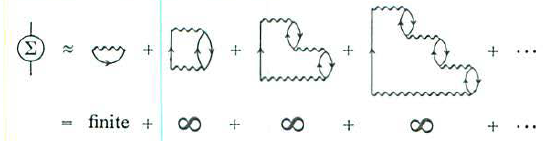
\includegraphics[width=0.8\textwidth]{screenshots/RPA-sigma.PNG}
    \label{RPA-sigma}
\end{equation}
The sum over rings is easy. Factoring out a free propagator from each diagram in (\ref{RPA-sigma}):
\begin{equation}
    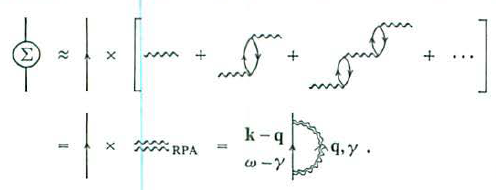
\includegraphics[width=0.8\textwidth]{screenshots/RPA-sigma-factor.PNG}
    \label{RPA-sigma-factor}
\end{equation}
T he double wiggle is the "\textbf{effective interaction}" in RPA
\begin{equation}
    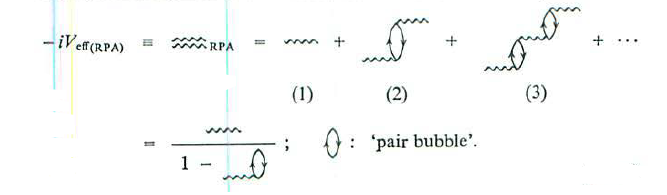
\includegraphics[width=0.8\textwidth]{screenshots/effective-RPA-factor.PNG}
    \label{effective-RPA-factor}
\end{equation}
Diagrams of form (1), (2), (3), ... , having one interaction line entering and one leaving are called '\redp{polarization diagrams}'. The reason for this is that they show how the interaction causes the medium to become 'virtually polarized' in all possible ways.

Equation (\ref{effective-RPA-factor}) may be written in functional form as
\begin{equation}V_{\mathrm{eff}(\mathrm{RPA})}(\mathrm{q}, \omega)=\frac{V_{q}}{1+V_{q} \pi_{0}(\mathrm{q}, \omega)}=\frac{V_{q}}{\epsilon_{\mathrm{RPA}}(\mathrm{q}, \omega)}
\label{Veff(RPA)}
\end{equation}
where
\begin{equation}
    -i\pi_0(\mathbf{q},\omega)\equiv\substack{\mathbf{k+q}\\\epsilon+\omega}\fermiloop\mathbf{k},\epsilon
\end{equation}
\bluep{This has the form of an interaction taking place between two charges in a dielectric, with}
\begin{equation}\epsilon_{\mathrm{RPA}}(q, \omega)=1+V_{q} \pi_{0}(\mathrm{q}, \omega)\end{equation}
\bluep{being the frequency-dependent or so-called 'generalized' dielectric constant}
\begin{mybox}
The dielectric properties of a medium arise just because of the polarization of the medium by a field, and (\ref{effective-RPA-factor}) is just the sum of diagrams representing the polarization of the electron gas by the field of one of the electrons in the gas itself.\textbf{ If $V_{\text {eff }}$ is Fourier transformed to $(q, t)$ -space, it will thus be a time-dependent interaction; this is due to the inertia of the polarization charge.}
\end{mybox}
We may evaluate $\pi_0(\mathbf{q},\omega)$ by
\begin{equation}-i \pi_{0}(\mathbf{q}, \omega)=2 \times(-1) \int \frac{d^{3} \mathbf{k} d \epsilon}{(2 \pi)^{4}} \frac{i}{\omega+\epsilon-c_{k+q}+i \delta_{k+q}} \times \frac{i}{\epsilon-\epsilon_{k}+i \delta_{k}}\end{equation}
where the factor of 2 comes from the sum over spins and the ( -1) from the fermion loop. In
the limit when $\omega$=O and $\mathbf{q}$ is small, it is found that
\begin{equation}\pi_{0}\left(q \ll k_{F}, \omega=0\right)=\frac{\lambda^{2}}{4 \pi e^{2}}, \quad \lambda^{2}=\frac{6 \pi n e^{2}}{\epsilon_{F}}=\frac{4 m e^{2} k_{F}}{\pi}=\left(\frac{2}{\pi}\right)\left(\frac{4}{9 \pi}\right)^{1 / 3} r_{s} k_{F}^{2}\end{equation}
where $n=$ electron density $=\frac{1}{3} \pi^{-2} k_{F}^{3}, \epsilon_{F}=k_{F}^{2} / 2 m$. Setting $\Omega=1$ and omitting spins for simplicity, we have \begin{equation}V_{q}=\frac{4 \pi e^{2}}{q^{2}}\end{equation}
Substituting $\pi_0$ and $V_q$ into (\ref{Veff(RPA)}) yields
\begin{equation}V_{\mathrm{eff}(\mathrm{RPA})}(\operatorname{small} \mathrm{q}, 0)=\frac{4 \pi e^{2}}{q^{2}+\lambda^{2}}\end{equation}

We can now go on to the evaluation of $\Sigma_{RPA}(\mathbf{k},\omega)$ as:
\begin{equation}\begin{aligned}
-i \sum_{\mathrm{RPA}}(\mathbf{k}, \omega) &=\sum_{\mathbf{q}} \int \frac{d \gamma}{2 \pi}\left[(-i) V_{\mathrm{eff}(\mathrm{RPA})}(\mathbf{q}, \omega)\right]\left[i G_{0}(\mathbf{k}-\mathbf{q}, \omega-\gamma)\right] \\
&=\int \frac{d^{3} \mathbf{q}}{(2 \pi)^{3}} \int \frac{d \gamma}{2 \pi} \frac{4 \pi e^{2}}{q^{2} \epsilon_{\mathrm{RPA}}(\mathbf{q}, \gamma)} \times \frac{1}{\omega-\gamma-\epsilon_{k-q}+i \delta_{k-q}}
\end{aligned}
\label{Sigma-RPA-int}
\end{equation}
